% =============================================================================
\section{Squeezing by component separation}
% =============================================================================

As an example of measurement of the degree of squeezing in a real two-component \abbrev{bec} system, we will consider a recent experiment~\cite{Riedel2010}, in which multi-particle entanglement and resulting spin squeezing was achieved by controlling nonlinear interaction using a component-dependent potential.

The experiment essentially consisted of the same regular Ramsey sequence as depicted in~\figref{bec-noise:visibility:sequences},~(a) performed for $1250$ \Rb{} atoms in the hyperfine state ${\ket{F=1,\, m_F=-1}}$ in a cigar-shaped trap with $f_x = f_y = 109\un{Hz}$, $f_z = 500\un{Hz}$.
The experiment started with an application of a $\pi/2$-pulse using an oscillator with the Rabi frequency $\Omega=2\pi \times 2.1\times 10^{3}\un{rad/s}$, creating an equal superposition of two hyperfine states ${\ket{F=1,\, m_F=-1}}$ and ${\ket{F=2,\, m_F=+1}}$.
The second pulse had a varied length allowing a measurement of the spin along the angle $\theta$: $\hat{S}_\theta = \hat{S}_z \cos \theta - \hat{S}_y \sin \theta$ (spin tomography).

The important difference was an addition of the component-dependent longitudinal shift to the potential $l_x^{(1,2)} = \pm 0.26\un{\mu m}$ right after the first pulse (as described by~\eqnref{bec-noise:system:V}), persisting the whole time of the evolution until the second oscillator pulse.
This effectively reduced the component overlap and provided a way of enabling the nonlinearity only at a chosen ``best squeezing'' time according to the one-axis twisting Hamiltonian model~\cite{Kitagawa1993}.

\begin{figure}
    \centerline{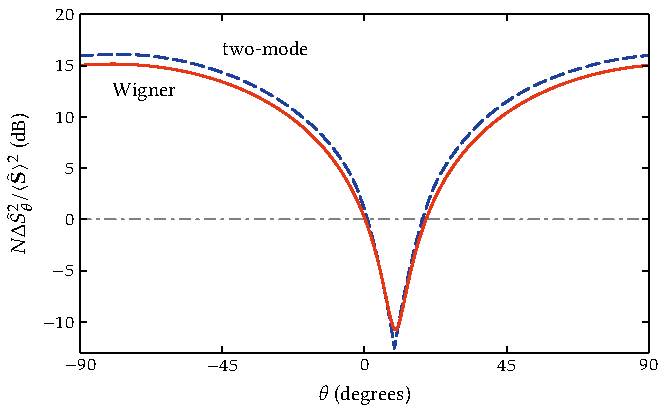
\includegraphics{figures_generated/bec_squeezing/riedel_rotation.pdf}}

    \caption[Wigner simulated spin tomography in the component separation experiment]{
    Dependence of the normalized variance of the total spin in the orthogonal plane on the rotation angle $\theta$ for the Wigner method (red solid line) and the two-mode variational method (dashed blue line, data taken from Riedel \textit{et~al}~\cite{Riedel2010}).
    }%endcaption
    \label{fig:bec-squeezing:separation:tomography}
\end{figure}

The truncated Wigner approach is applied straightforwardly to this system and allows us to measure the degree of squeezing $\xi^2$ according to the formula~\eqnref{bec-squeezing:theory:xi2}, calculating the required spin correlations using the expressions derived in \secref{bec-squeezing:theory}.
Furthermore, we can simulate the observations closer to those used in the experiment, and collect the spin tomography results, as shown in~\figref{bec-squeezing:separation:tomography}.
The maximum degree of squeezing and the corresponding rotation angle corresponds to the minimum of the graph.

The Wigner method shows good agreement with the two-mode variational method~\cite{Li2009}, which was used by the experimental team, and also includes the effect of particle losses.
The two-mode method predictions were taken from~\cite{Riedel2010} and plotted in~\figref{bec-squeezing:separation:tomography} for the sake of comparison.
The figure demonstrates that the predictions of the two methods for the maximum squeezing angle are nearly identical, and the predictions of the degree of squeezing are close, yet noticeably different ($-10.73\pm0.05\un{dB}$ from the Wigner method as compared with $-12.8\un{dB}$ from the two-mode method).
We believe that this is caused by the Wigner method being a more systematic type of quantum noise treatment, and, consequently, more suitable for such complex calculations.

This prediction is hard to verify experimentally as the technical noise greatly reduces the degree of squeezing (down to $-3.7\un{dB}$), moving it far from the theoretical limit.
The technical noise was not included in the simulations in this thesis, although it can be done similarly to \charef{bec-noise} (since the technical noise in this experiment has similar nature).
On the other hand, the maximum ``unsqueezing'' (the maximums of the plot in~\figref{bec-squeezing:separation:tomography}), while being irrelevant for practical purposes, can serve as a good experimental check for the two-mode and Wigner methods, as it is much less affected by the technical noise.
The difference of $1\un{dB}$ in the maximum unsqueezing between the two methods should be possible to distinguish.

\begin{figure}
    \centerline{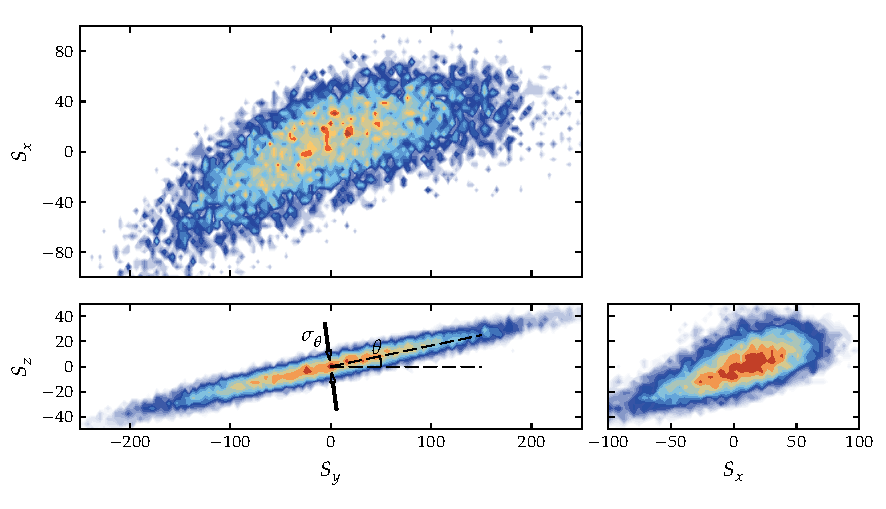
\includegraphics{figures_generated/bec_squeezing/riedel_cloud.pdf}}

    \caption[Orthogonal projections of total spin uncertainty cloud]{
    Reconstructed probability distribution for the components of the total spin vector in $xy$ (top), $yz$ (bottom left) and $xz$ (bottom right) planes.
    The $yz$ plane illustrates the spin squeezing achieved in the experiment: the variance $\Delta^2 \hat{S}_\theta$ is the variance of the distribution in the direction $\theta$ (shown with two arrows): $\Delta^2 \hat{S}_\theta \equiv \sigma_\theta^2$.}%endcaption
    \label{fig:bec-squeezing:separation:cloud}
\end{figure}

We can go further and reconstruct the spin noise distribution using per-path values of the total spin components, as explained in the end of \secref{bec-squeezing:theory}.
The projections of the resulting probability distribution on three orthogonal planes are shown in~\figref{bec-squeezing:separation:cloud}.
The projection on the $yz$ plane is similar to the one obtained experimentally~\cite{Riedel2010}, and it is clearly seen that the direction used to measure the squeezing in the experiment is indeed the best one, as the cloud is much wider in other directions.
The $yz$ pane illustrates the physical meaning of the best squeezing angle: it is chosen so that the standard deviation of the total spin distribution in the orthogonal direction is minimal.
